\scanpage{78}
$f$. For instance, using Chow's lemma and the Main existence theorem in my first talk on Picard schemes, one gets:

\uline{Corollary} 2\quad Assume $X/S$ proper satisfies the condition:\deleted{\unsure{a') for every}} \deleted{\unsure{any $X'$}\illegible{2} for} a') for every $X'$ finite over $X$, there \unsure{exist|exists} a non empty open subset $S_1$ of $S$ such that \inserted{\handwritten{problem A for}} $X'\handwritten{\mid}S_1$ has allways solution \deleted{for problems A and B} (this condition is satisfied if $X/S$ is projective). Then \deleted{there exists} provided we replace $S$ by a suitable $S_1$ non empty and open, $\underline{\mathrm{Pic}}_{X/S}$ exists, is separated, its connected components are of finite type over $S$.

N.B. The proof does not give any evidence towards the fact that in the theorem, one could replace ``quasi-affine'' by ``affine'' . This is true however over a \unsure{fiéèd|fièèd|field}, because a quasi-affine algebraic group is affine ! It would be interesting to have a couterexample, say,over a \deleted{valuation} ring of dimension $1$ such as $k\handwritten{[}t\handwritten{]}$ , $X$ and $X'$
\figure{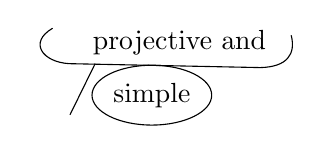
\begin{tikzpicture}[x=1cm,y=1cm]
\node[inner sep=0pt] (addition) at (0.35,0.67) {\inserted{projective and}};
\node[inner sep=0pt] (simple) at (0,0) {simple};
\handwritten{\draw (simple.center) ellipse (0.76cm and 0.38cm);
\draw (-1.26,0.85) .. controls (-1.57,0.67) and (-1.39,0.42) .. (-1.05,0.40) -- (1.38,0.35) .. controls (1.72,0.36) and (1.83,0.52) .. (1.77,0.76);
\draw (-0.72,0.40) -- (-1.04,-0.25);}
\end{tikzpicture}}\margin{\handwritten{\figure{
\begin{tikzpicture}\draw (0,0) ellipse (0.25cm and 0.18cm);\end{tikzpicture}}impossible if\\$X$ smooth!}}
% The N.B. paragraph continues across this source drawing.
over $S$ and $X'\handwritten{\to}X$ birational,\unsure{or\deleted{r}|orr|orx} alternatively, \deleted{\unsure{if $X'$ finite}} $X$ and $X'$ projective and normal over $S$, and $f:X'\handwritten{\to}X$ finite. A counterexample in the latter case would of course provide a couterexample to the effectivity
% In the source line the circled phrase stands at the right; its connector attaches it immediately after problem(s). Node declaration order follows that attachment.
\figure{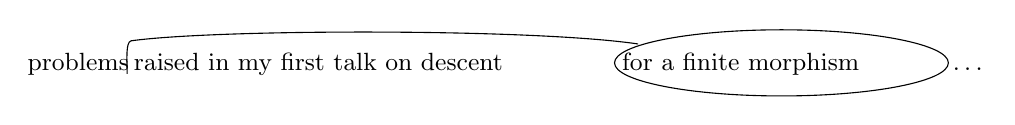
\begin{tikzpicture}[x=1cm,y=1cm,every node/.style={font=\small,inner sep=0pt,anchor=base west}]
\node (problem) at (0,0) {problem\deleted{\unsure{s}}};
\node (moved) at (7.55,0) {\inserted{for a finite morphism}};
\node (raised) at (1.35,0) {raised in my first talk on descent};
\node at (11.75,0) {\dots};
\handwritten{\draw (9.58,0.10) ellipse (2.12cm and 0.42cm);
\draw (7.76,0.34) .. controls (6.40,0.54) and (2.40,0.53) .. (1.32,0.38) .. controls (1.25,0.36) and (1.27,0.15) .. (1.27,-0.04);}
\end{tikzpicture}}

``Problem A'' is the following: given $X/S$ and \deleted{any} Module $F$ on $X$, to represent the functor on the category of $S$-preschemes taking any $S'/S$ into \deleted{the empty or} into a one-element \inserted{or into the empty} set; according as to whether $F'$ on $X'/S'$ is flat with respect to $S'$\inserted{\handwritten{or not}}, where $X'=X\mathbin{x}_S S'$, $F'=F\unsure{2|x|\otimes}_S S'$ . Given $X/S$, we say that ``Problem A \inserted{\handwritten{for $X/S$}} has always a solution'' if for every coherent $F'$ on \deleted{$X$}\inserted{\handwritten{some $X'/S'$}}, the previous functor \inserted{\handwritten{on $(\mathrm{Sch})/S'$}} is representable by a \inserted{$S\handwritten{'}$\handwritten{-}}scheme of finite type. The main step in my proof of existence of Hilbert schemes shows that this condition is satisfied when $X/S$ is projective,
% archive sheet number: 77
